%
% Article for Security RSA Cryptography
% Writed by: Stavros Papantonakis
%
%!TEX TS-program = xelatex
%!TEX encoding = UTF-8 Unicode
%
\documentclass[a4paper,12pt]{article}
	\usepackage{fontspec,xltxtra,xunicode}
	% Begin new paragraphs with an empty line rather than an indent
	\usepackage[greek]{babel}
	% justify paragraphs
	\usepackage[parfill]{parskip}
	\usepackage{xgreek}    
	%\usepackage{url}
	\usepackage{multirow}
	\usepackage{fancyvrb}
	\usepackage{colortbl}
	\usepackage{anyfontsize}
	\usepackage[usenames,dvipsname]{xcolor}
	\usepackage[colorlinks=true,linkcolor=black]{hyperref}
	\usepackage{pdfpages}
	\usepackage{ragged2e}
	\usepackage{babel}
	\usepackage{listings}
	\usepackage{amsmath}
	\usepackage{centernot}
	% Scaling based on Scale=MatchLowercase and Times New Roman
	% causes inconsistent output between OS X and FreeBSD
	% Therefore Scale is now set as an absolute number
	%\defaultfontfeatures{Scale=0.975,Mapping=tex-text}

	\newif\ifextrachapters
	
	
	%\defaultfontfeatures{Mapping=tex-text}	
	%\setromanfont[Mapping=tex-text]{Times New Roman}	
	\setmainfont[Mapping=tex-text]{GFS Didot}
	
	\usepackage{multicol}
	\usepackage{graphicx}
	\setcounter{secnumdepth}{4}
	\setcounter{tocdepth}{4}
	\usepackage{fancyhdr}
	\pagestyle{fancy}
	\fancyhf{}

	\fancyhead[LE,RO]{\bfseries\thepage}
	\fancyhead[LO]{\bfseries\rightmark}
	\fancyhead[RE]{\bfseries\leftmark}

	\renewcommand{\headrulewidth}{0.5pt}
	\addtolength{\headheight}{2pt}
	\renewcommand{\footrulewidth}{0pt}
	\addtolength{\headheight}{0.5pt}
	
	\fancypagestyle{plain}{%
	\fancyhead{}
	\renewcommand{\headrulewidth}{0pt}}
	
	%
	% User defined environments and commands
	%
	\newenvironment{inthebox}{\line(1,0){390}\\} %
  		{\line(1,0){390}}
	\DefineVerbatimEnvironment{richverb}%
		{Verbatim}{commandchars=\|\[\], commentchar=\!}
	\newcommand{\boxline}{\line(1,0){390}\\}	
	
	\author{Παπαντωνακης Σταυρος}
	\title {Arduino Fire Car}
	\date{7/4/2020}
	%
	%	
\begin{document}
	%
	%\maketitle
	% Title page
	%
	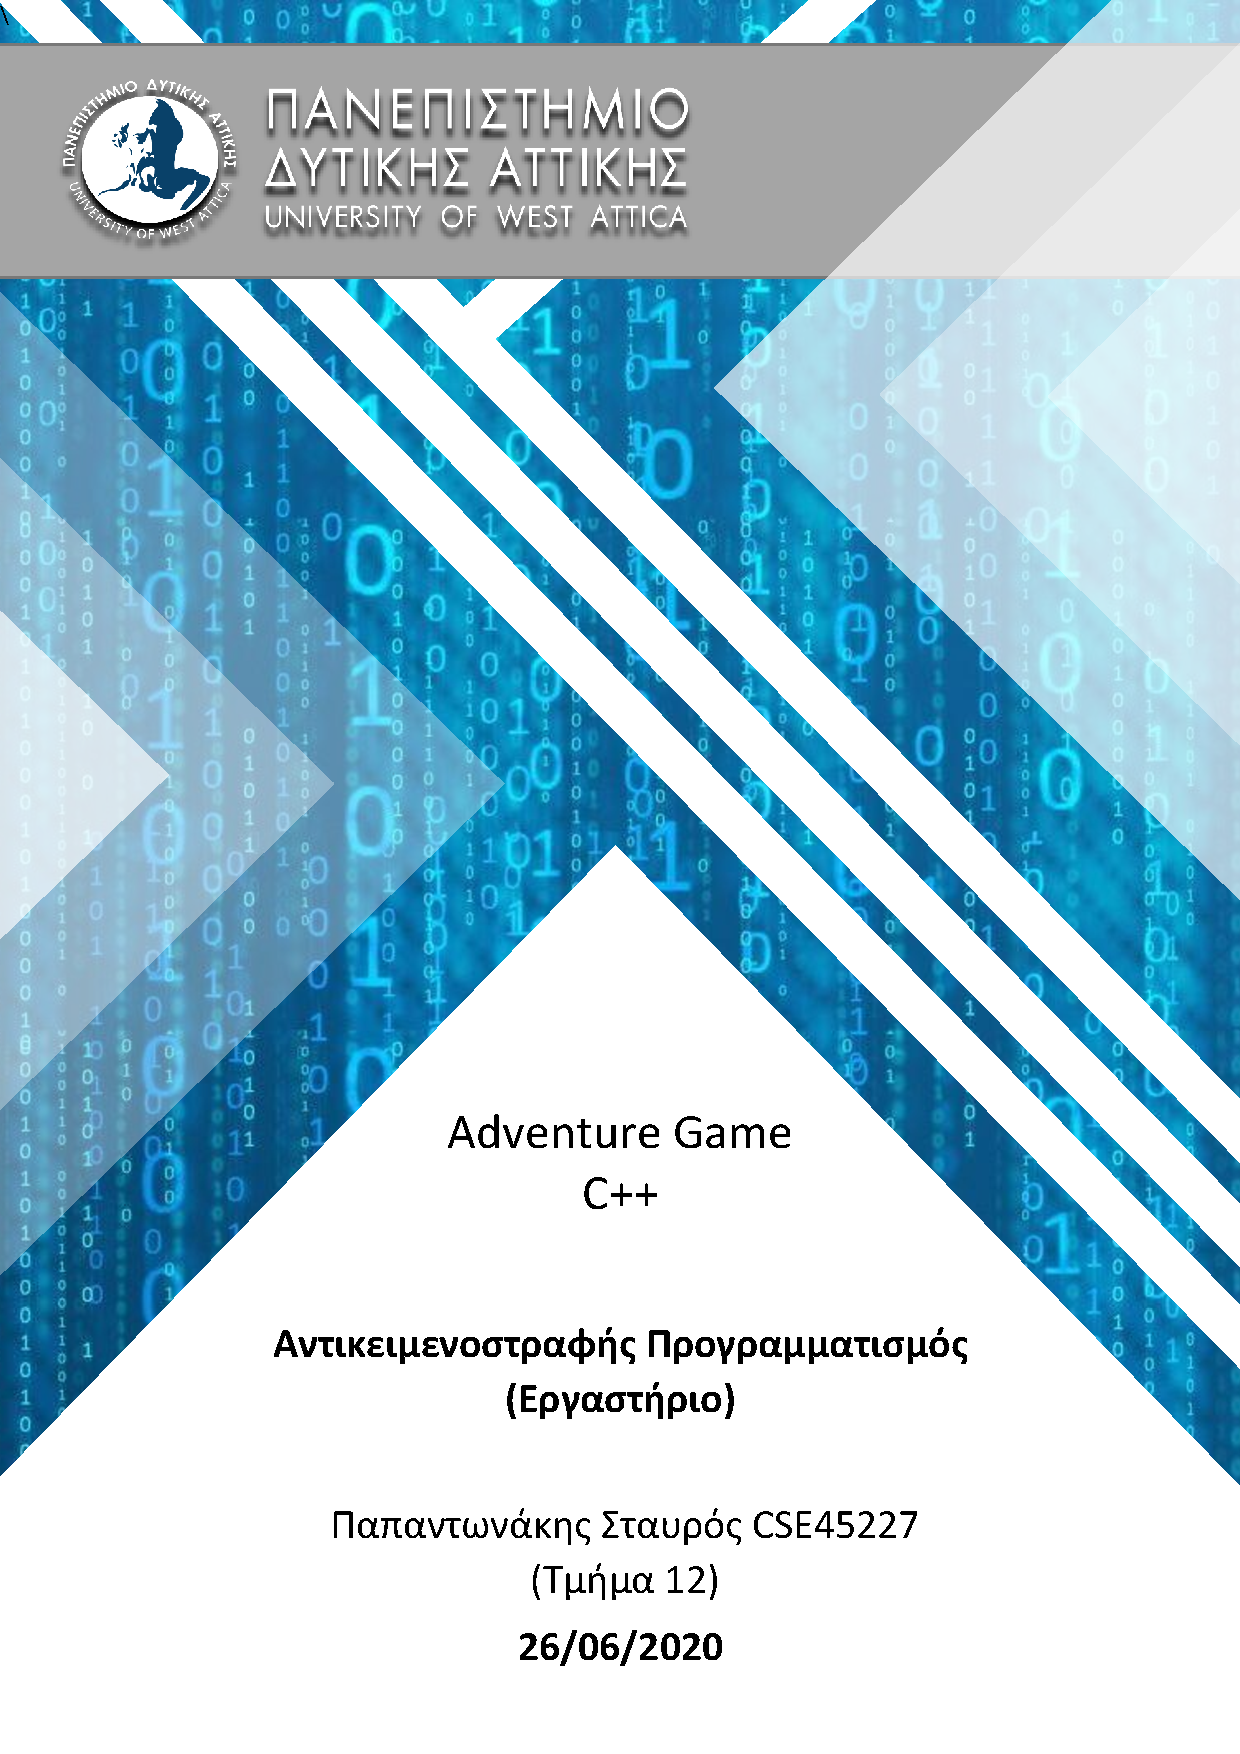
\includepdf[pages=-]{cover/cover}
	%
% Writed by: Stavros Papantonakis
%
%!TEX TS-program = xelatex
%!TEX encoding = UTF-8 Unicode
%
\begin{titlepage}
	\begin{center}
		\vspace{1cm}	
		\Huge	
		\textbf{Adventure Game}
		
		\vspace{0.5cm}
		\large
		Αντικειμενοστραφής σχεδιάσει ενός Adventure παιχνιδιού στην γλωσσά C++
				
		\vspace{1.5cm}
		\textbf{Παπαντωνάκης Σταύρος\\ CSE45227}
		\vfill
		
		Αναφορά τελικής εργασίας \\
		Τμήμα 12
		\vspace{0.8cm}
		\begin{center}
			
\includegraphics[width=0.4\textwidth]{image/logo.jpg}		
		\end{center}
		\normalsize
		Τμήμα Μηχανικών Πληροφορικής και Υπολογιστών\\
		Πανεπιστήμιο Δυτικής Αττικής\\
		Αθηνά\\
		26/06/2020\\	
	\end{center}
\end{titlepage}
	%
	% Creative Commons 4.0 License
	%
	%
% CC 4.0 License translation test file
% Translated by: Manolis Kiagias
%
%!TEX TS-program = xelatex
%!TEX encoding = UTF-8 Unicode
%
\begin{center}
Copyright \copyright 2020 Παπαντώνακης Σταύρος\\
Το Παρόν Έργο παρέχεται υπό τους όρους της Άδειας:\\

\includegraphics[scale=0.2]{license/images/cc-logo}\\
\textbf{Αναφορά Δημιουργού-Μη Εμπορική Χρήση-Παρόμοια Διανομή 4.0 Διεθνής}\\
Το πλήρες κείμενο αυτής της άδειας είναι διαθέσιμο εδώ:\\
\url{http://creativecommons.org/licenses/by-nc-sa/4.0/}
\end{center}
\subsection*{Είστε ελεύθερος να:}
\noindent
\textbf{Διαμοιραστείτε} -- να αντιγράψετε και αναδιανείμετε το υλικό με οποιοδήπότε μέσο και μορφή.\\
\textbf{Προσαρμόσετε} -- να αναμείξετε, μετασχηματίσετε και να επεκτείνετε το υλικό.\\

Ο αδειοδότης δεν μπορεί να σας αφαιρέσει αυτές τις ελευθερίες όσο ακολουθείτε τους όρους της παρούσας άδειας.
\subsection*{Ύπο τους ακόλουθους όρους:}

\vspace{1em}
\noindent
\parbox{1.5cm}{
\includegraphics[scale=0.15]{license/images/cc_by_30}}
\parbox{10.5cm}{\textbf{Αναφορά Δημιουργού} -- Θα πρέπει να αναφέρετε \textbf{τον δημιουργό του έργου}, να παρέχετε σύνδεσμο προς αυτή την άδεια, και να \textbf{υποδείξετε τυχόν αλλαγές}. Μπορείτε να το κάνετε με οποιοδήποτε εύλογο μέσο, αλλά όχι με τρόπο που να υπονοεί ότι ο αδειοδότης επικροτεί εσάς ή τη χρήση του έργου από εσάς.}

\vspace{1em}
\noindent
\parbox{1.5cm}{
\includegraphics[scale=0.15]{license/images/cc_nc_30}}
\parbox{10.5cm}{\textbf{Μη Εμπορική Χρήση} --  Δεν μπορείτε να χρησιμοποιήσετε το υλικό για \textbf{εμπορικούς σκοπούς}.}

\vspace{1em}
\noindent
\parbox{1.5cm}{
\includegraphics[scale=0.15]{license/images/cc_sa_30}}
\parbox{10.5cm}{\textbf{Παρόμοια Διανομή}  -- Αν αναμείξετε, μετασχηματίσετε ή επεκτείνετε το υλικό, θα πρέπει να διανείμετε τις αλλαγές σας υπό την \textbf{ίδια άδεια} με το πρωτότυπο έργο.}

\vspace{1em}
\noindent
\parbox{1.5cm}{\ }
\parbox{10.5cm}{\textbf{Όχι επιπλέον περιορισμοί} -- Δεν μπορείτε να εφαρμόσετε νομικούς όρους ή \textbf{τεχνικά μέσα} που να περιορίζουν νομικά τους άλλους να πράξουν σύμφωνα με τις ελευθερίες αυτής της άδειας.}
\subsection*{Σημειώσεις:}
\noindent
Δεν χρειάζεται να ακολουθήσετε την άδεια για τμήματα του υλικού που θεωρούνται δημόσια γνώση (public domain) ή όπου η χρήση τους επιτρέπεται εξαιτίας μιας \textbf{εξαίρεσης ή περιορισμού}.\\

\noindent
Δεν δίνονται εγγυήσεις. Η άδεια ίσως να μη σας δίνει όλα τα δικαιώματα για την επιδιωκόμενη χρήση. Για παράδειγμα, επιπλέον δικαιώματα όπως \textbf{δημοσιότητα, ιδιωτικότητα, ή ηθικά δικαιώματα} μπορεί να επιβάλλουν περιορισμούς στη χρήση του υλικού.\\
\line(1,0){390}\\\\
\noindent
Το παρόν έργο στοιχειοθετήθηκε σε \XeLaTeX. Ο πηγαίος κώδικας του είναι διαθέσιμος στην παρακάτω τοποθεσία:
\begin{center}
\url{https://github.com/lardianos/Adventure}
\end{center}
\newpage	
	%
	%
	\tableofcontents		
	\newpage
	% Writed by: Stavros Papantonakis
%
%!TEX TS-program = xelatex
%!TEX encoding = UTF-8 Unicode
%
\section*{Εισαγωγή}
%Aferesi kenou arxis paragrafou
\noindent
"Όπως μας ζητήθηκε από την εταιρεία eFUN A.E" αναπτύξαμε την βασική δομή
ενός παιχνιδιού της κατηγορίας adventure. Η δομή του παιχνιδιού καθώς και 
το σενάριο του αφέθηκε στην φαντασία μας, η μονή απαίτηση που υπήρξε είναι να τηρεί τους κανόνες της αντικειμενοστραφείς σχεδιάσεις καθώς και κάποια τεχνικά
ζητήματα συμπεριλαμβανόμενου της ανακτήσεις και αποθηκεύσεις δεδομένων του παιχνιδιού. 


	
	% Writed by: Stavros Papantonakis
%
%!TEX TS-program = xelatex
%!TEX encoding = UTF-8 Unicode
%
\setcounter{section}{0}
\section{Σενάριο Παιχνιδιού}


\noindent
Η ιστορία του παιχνιδιού διαδραματίζετε σε ένα δάσος, όπου ο πρωταγωνιστής
μας έχει βρεθεί. Το δάσος είναι σκοτώνω καθώς επικρατεί παντού η νύχτα και ο 
χαρακτήρας μας πεινάει καθώς δεν ξέρει πως βρέθηκε εκεί, πόσες μέρες έχουν
περάσει και πως θα φύγει. Το μόνο πράγμα που έχει μαζί του είναι ένα μαγικό 
σακίδιο που χωράει 10 αντικείμενα οποιουδήποτε μεγέθους. Σκοπός του χαρακτήρα
που χειριζόμαστε είναι να καταφέρει να φάει για να επιβιώσει. Για να το πετύχει αυτό θα πρέπει ναι περιηγηθεί στο δασός την νύχτα με όσους κινδύνους και αν κρύβει αυτό να συλλέξει όσα περισσότερα αντικείμενα μπορεί και να χρησιμοποιήσει την ευφυΐα του και τις γνώσεις που διαθέτει για να κατασκευάσει εργαλεία και αντικείμενα που θα τον βοηθήσουν να πετύχει τον σκοπό του. Το σακίδιο του περιεχέι αρχικά ένα πακέτο με σπίρτα και ένα μαχαίρι.

\section{Περιβάλλον Και Αντικείμενα}
\noindent
Το διαθέτει 4 χορούς στους οποίους μπορούμε να περιηγηθούμε. Οι χοροί αυτοί είναι ο χώρος του δάσους που εμφανιζόμαστε για πρώτη φορά, ένα ξέφωτο, μια λίμνη και ένα μέρος του δάσους με πολύ πυκνούς θάμνους.

Σε καθένα από αυτούς τους χώρους/περιβάλλοντα  υπάρχουν σκορπισμένα αντικείμενα που αναζητώντας τα μπορούμε να τα συλλέξουμε και να τα συνδυάσουμε για να δημιουργήσουμε νέα αντικείμενα.

Ο παρακάτω χάρτης θα μας βοηθήσει να καταλάβουμε πως είναι δομημένα τα περιβάλλοντα.

\begin{center}
			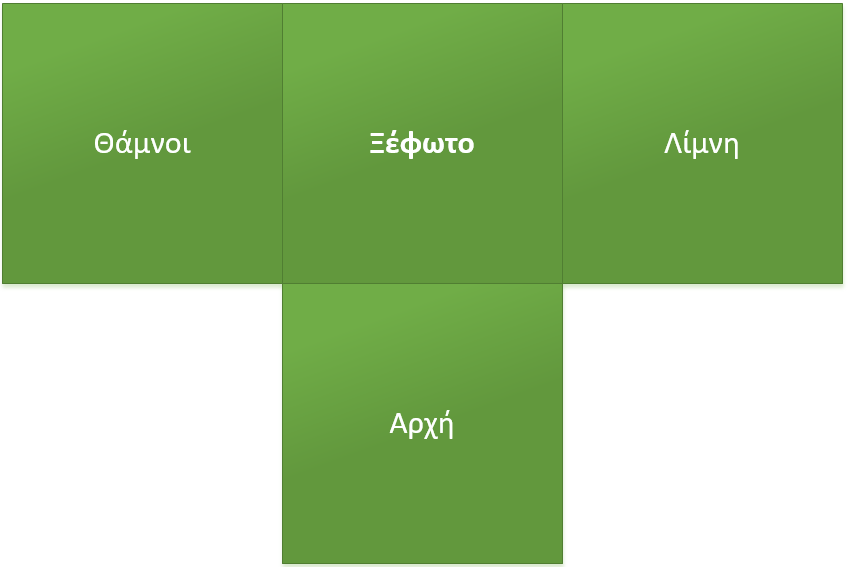
\includegraphics[width=1\textwidth]{image/1.1.PNG}		
\end{center}
\noindent 
Έχουμε κωδικοποιήσει τα περιβάλλοντα με έναν αύξων αριθμό το οποίο χρησιμοποιούμε για να ξέρουμε κάθε φορά σε ποιο περιβάλλον βρισκόμαστε.

\begin{center}
			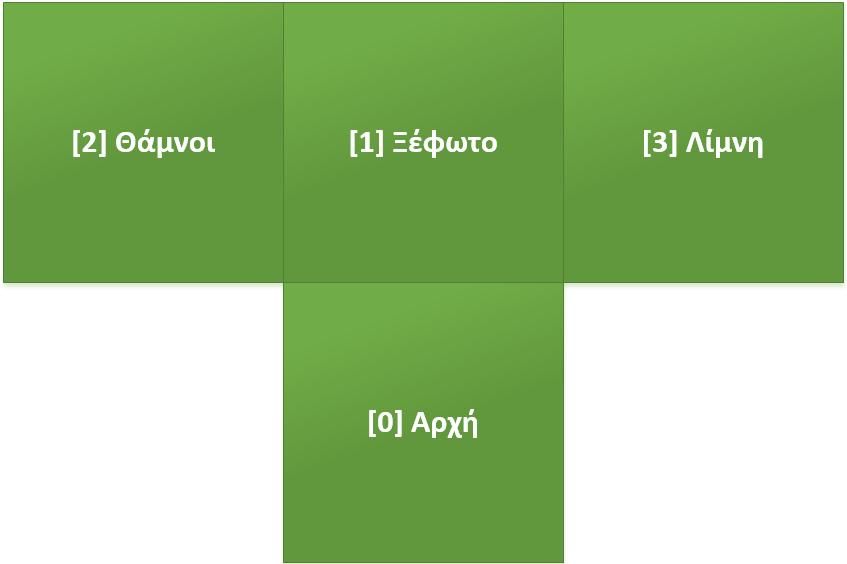
\includegraphics[width=1\textwidth]{image/1.2.PNG}		
\end{center}

\noindent
Τα αντικείμενα που υπάρχουν η μπορούν να υπάρξουν στο παιχνίδι είναι τα εξής.

\begin{center}
	\begin{lstlisting}	
0001;Σπίρτα;1
0002;Σχοινί;1
0003;Μαχαίρι;0
0004;Ξύλο;1
0005;Βέλος;1
0006;Τόξο;1
0007;Οπλισμένο Τόξο;1
0008;Ελάφι;0
0009;Κρέας;1
0010;Φωτιά;1
0011;Μαγειρεμένο Κρέας;1
	\end{lstlisting}	
\end{center}

\noindent
Από τα οποία μέσα στων χώρο του παιχνιδιού βρίσκονται μερικά από αυτά.

\begin{center}
			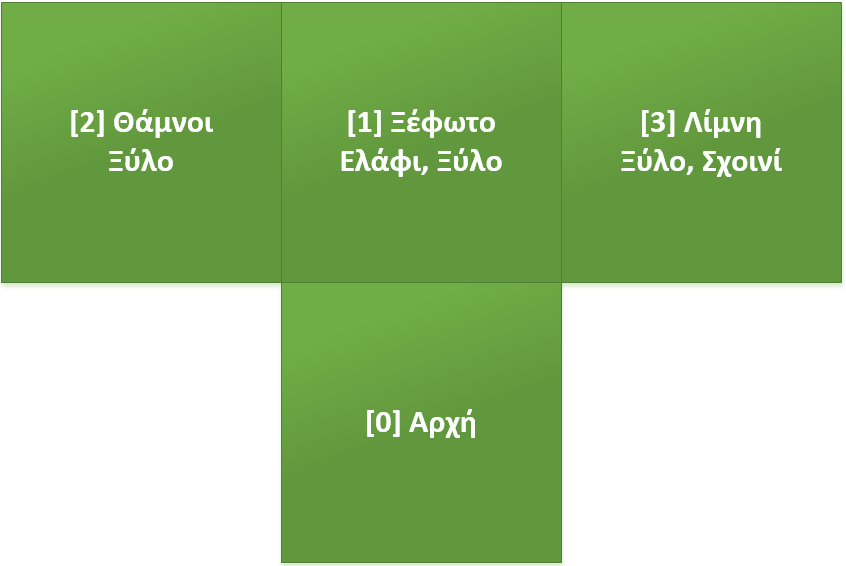
\includegraphics[width=1\textwidth]{image/1.3.PNG}		
\end{center}


\newpage
\section{Περιγραφή Αρχείου Εισόδου}
\subsection*{Απάντηση:}

\noindent
Για το αρχείο εισόδου έχουμε χρησιμοποιήσει την παρακάτω δομή.

\noindent
items\\
0001;Σπίρτα;1\\
0002;Σχοινί;1\\
0003;Μαχαίρι;0\\
0004;Ξύλο;1\\
0005;Βέλος;1\\
0006;Τόξο;1\\
0007;Οπλισμένο Τόξο;1\\
0008;Ελάφι;0\\
0009;Κρέας;1\\
0010;Φωτιά;1\\
0011;Μαγειρεμένο Κρέας;1\\
moves\\
1;-1;-1;-1\\
-1;0;3;2\\
-1;-1;1;-1\\
-1;-1;-1;1\\
buckpuck\\
0001\\
0003\\
0004\\
roomdesc\\
0;Βρίσκεσαι στο δάσος. Παντού σκοτάδι. Πίνας, κάτι πρέπει να κάνεις\\
1;Βρίσκεσαι σε ένα ξέφωτο. Έχει πανσέληνό, στο βάθος διακρίνεις ένα ελάφι. Είναι πολλή γρήγορο για εσένα\\
2;Βρίσκεσαι σε ένα πυκνό θάμνο. Ακούς έναν τρομαχτικό θόρυβο\\
3;Βρίσκεσαι σε μια λίμνη. Κάποιος έχει ξεχάσει κάτι στην όχθη της\\
roomitems\\
1;0004\\
1;0008\\
2;0004\\
3;0004\\
3;0002\\
\newpage
concatenate\\
0004;0003;0005\\
0002;0004;0006\\
0005;0006;0007\\
0008;0007;0009\\
0004;0001;0010\\
0009;0010;0011\\
winItems\\
0011\\

\noindent
items\\
Κάθε αντικείμενο έχει έναν κωδικό αντικείμενου και ένα όνομα καθώς και μια bool τιμή 0 η 1 για το αν αυτό το αντικείμενο μπορεί να μετακινηθεί η είναι στατικό.

\noindent
moves\\
Σε αυτό το σημείο έχουμε κωδικοποιήσει τις κινήσεις που μπορεί να κάνει
ο χαρακτήρας έτσι ώστε να μεταβεί από τον ένα χώρο στον επόμενο. Αρχικά 
σκευαστήκαμε να χρησιμοποιήσουμε τοις 4 κατευθύνσεις του ορίζοντα (Βοράς, Νότος, Ανατολή, Δύση) επόμενος φτιάξαμε 4 στήλες. κάθε στήλη αντιστοιχεί και σε μια κατεύθυνση. Στης κατευθύνσεις που δεν μπορούμε να πάμε βάζουμε την τιμή -1 ενώ στις υπόλοιπες βάζουμε των αριθμό του περιβάλλοντος που θα καταλήξουμε αν πάρουμε αυτήν την κατεύθυνση. Σε κάθε χώρο αντιστοιχεί μια γραμμή. Επόμενος παρατηρώντας την πρώτη γραμμή (1;-1;-1;-1) βλέπουμε ότι μπορούμε να πάμε μόνο προς των βορά και αν πάμε προς τα εκεί θα οδηγηθούμε
στον χώρο 1, αντίστοιχα στη δεύτερη γραμμή (-1;0;3;2) βλέπουμε ότι μπορούμε 
να πάμε νοτιά, ανατολικά και δυτικά άλλα όχι βόρια. Αν πάμε νοτιά θα οδηγηθούμε στον χώρο 0, ανατολικά στον χώρο 3 και δυτικά στον χώρο 2. Αντίστοιχα και για τους υπολοίπους χώρους.

\begin{center}
			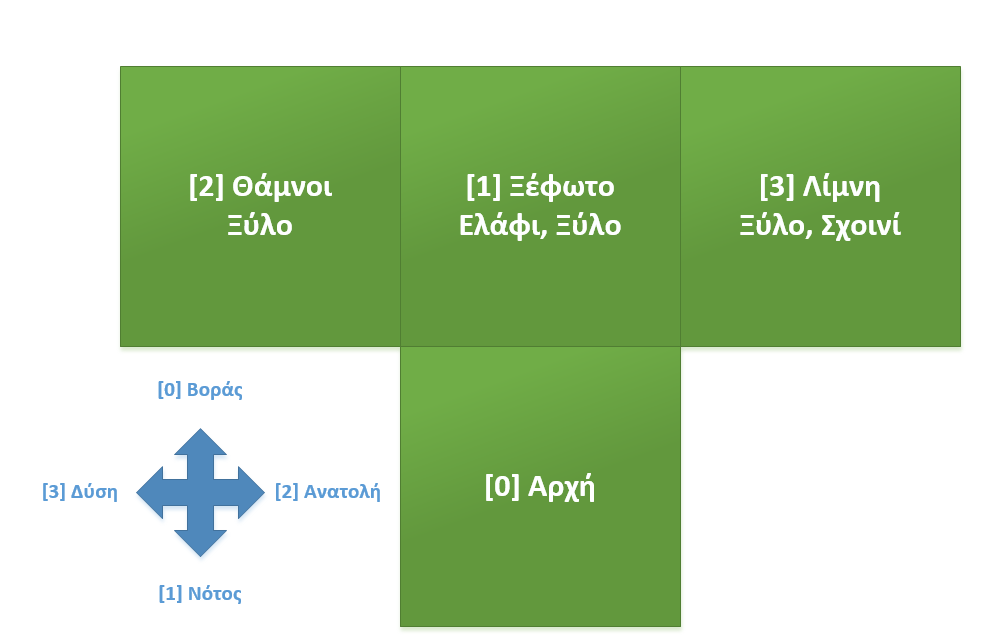
\includegraphics[width=1\textwidth]{image/1.4.PNG}		
\end{center}

\noindent
buckpuck\\
Εδώ βάζουμε τους κωδικούς αντικείμενων που θα βρισκόντανε αρχικά στο σακίδιο μας.

\noindent 
roomdesc\\
Σε αυτό το σημείο βάζουμε την περιγραφή και των κωδικό του κάθε χώρου.

\noindent
roomitems\\
Εδώ γράφουμε τη αντικείμενα υπάρχουν στον κάθε χώρο με τον κωδικό τους και 
τον κωδικό του χώρου.

\noindent
concatenate\\
Γράφουμε τους κανόνες δημιουργίας νέων αντικείμενων, πρώτη στήλη κωδικός
αντικείμενου 1 δεύτερη στήλη κωδικός αντικείμενο 2, τρίτη στήλη κωδικός νέου αντικείμενου. Οι συνδυασμού που έχουμε περιγράψει είναι οι εξής.

\noindent
Ξύλο + Μαχαίρι = Βέλος\\
Σχοινί + Ξύλο = Τόξο\\
Τόξο + Βέλος = Οπλισμένο Τόξο\\
Ελάφι + Οπλισμένο Τόξο = Κρέας\\
Ξύλο + Σπίρτα  = Φωτιά\\
Κρέας + Φωτιά = Μαγειρεμένο Κρέας\\

\noindent
winItems\\
Τέλος στο εδώ βάζουμε τα αντικείμενα που όταν κατασκευάσουμε κερδίζουμε. στην 
περίπτωση μας είναι το "Μαγειρεμένο Κρέας".

\section{Διαγράμματα Κλάσεων}
\subsection*{Απάντηση:}
\noindent

\begin{center}
			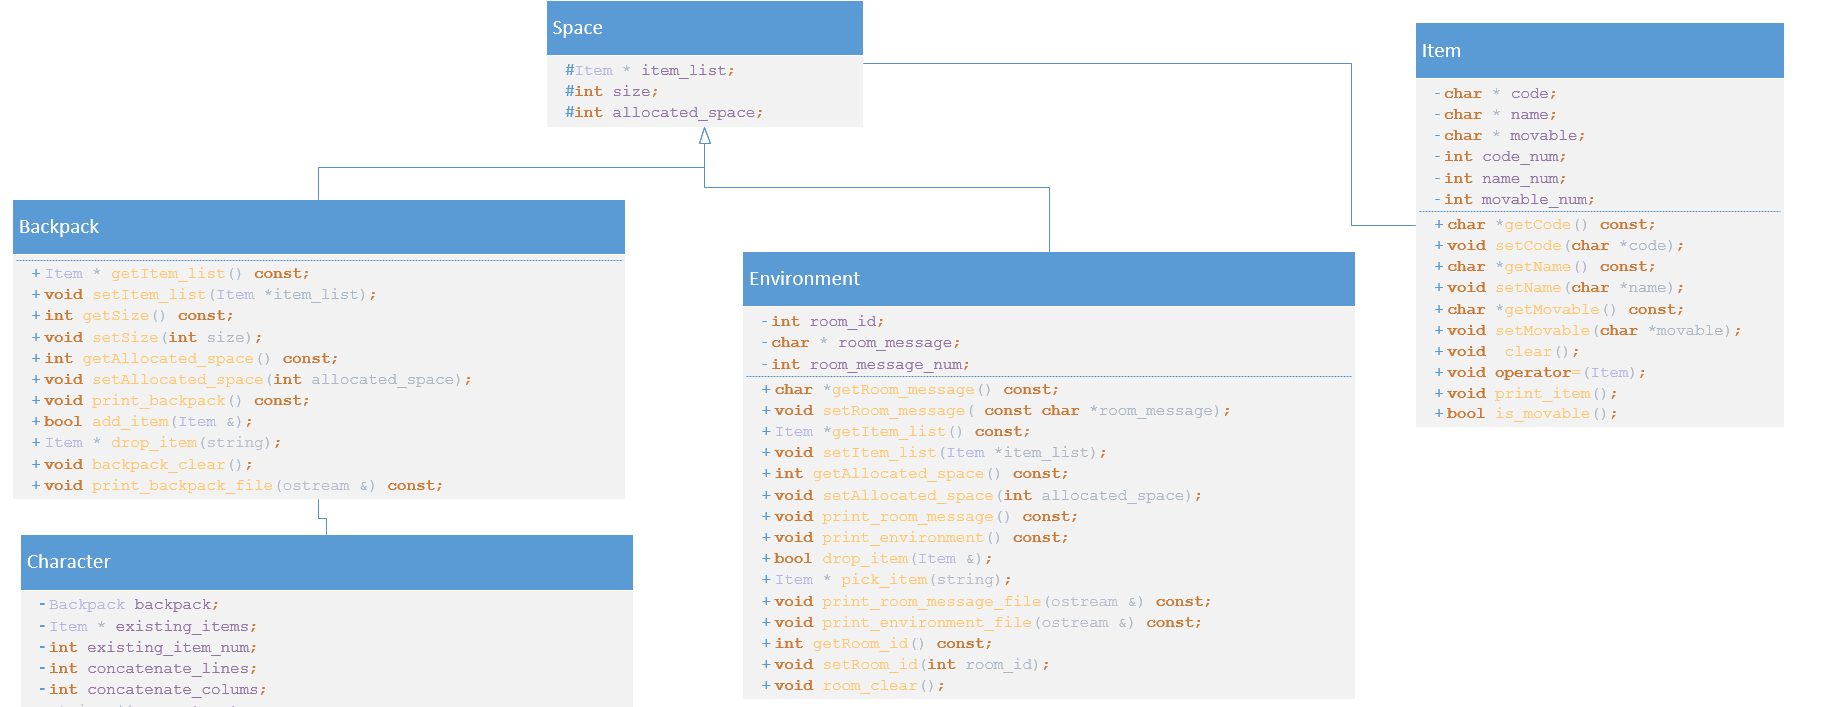
\includegraphics[width=1\textwidth]{image/1.5.0.PNG}		
\end{center}

\begin{center}
			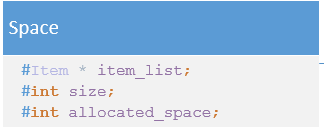
\includegraphics[width=1\textwidth]{image/1.5.1.PNG}		
\end{center}

\begin{center}
			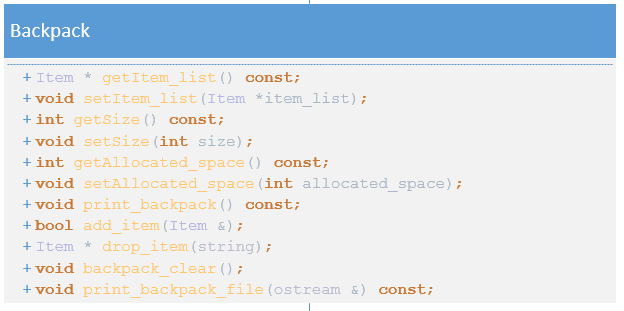
\includegraphics[width=1\textwidth]{image/1.5.2.PNG}		
\end{center}

\begin{center}
			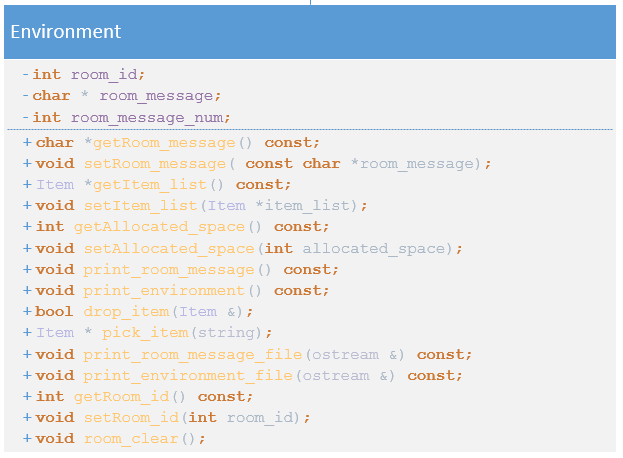
\includegraphics[width=1\textwidth]{image/1.5.3.PNG}		
\end{center}

\begin{center}
			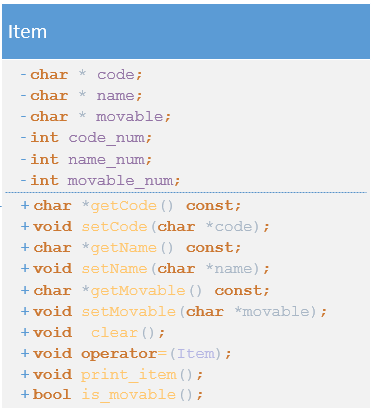
\includegraphics[width=1\textwidth]{image/1.5.4.PNG}		
\end{center}

\begin{center}
			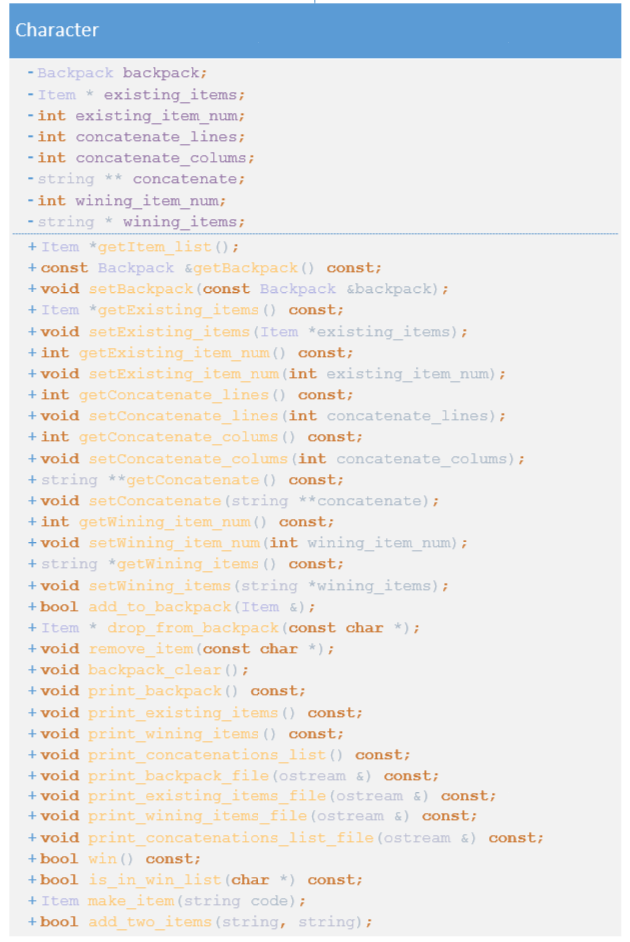
\includegraphics[width=1\textwidth]{image/1.5.5.PNG}
\end{center}

\section{Περιγραφή Σεναρίου Χρήσης}
\subsection*{Απάντηση:}

\noindent
Αρχικά ο χρήστης τρέχει το παιχνιδίζει ./a.out, του ζητείται να πληκτρολογήσει ένα αρχείο εισόδου. Για παράδειγμα πληκτρολογεί rooms.txt, το παιχνίδι φορτώνει τα δεδομένα και αρχίζει το παιχνίδι.

\noindent
Εμφανίζετε η παρακάτω οθόνη.
\begin{center}
			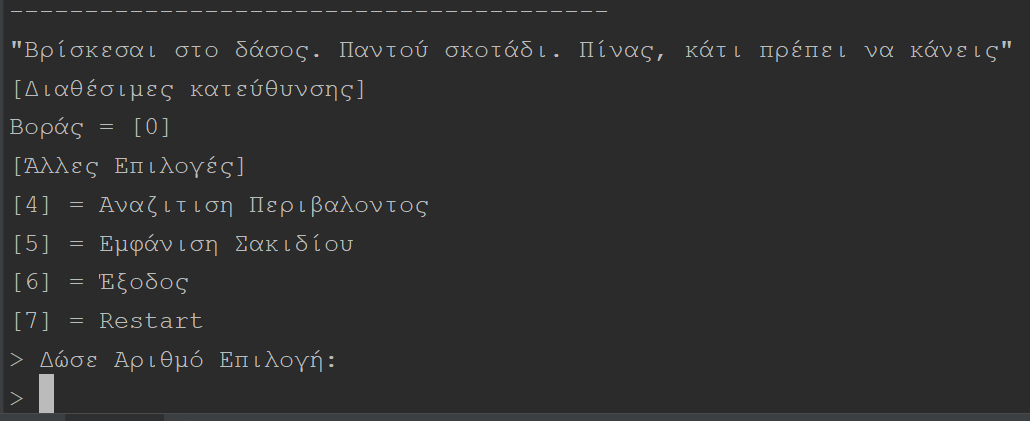
\includegraphics[width=1\textwidth]{image/2.1.PNG}
\end{center}

\noindent
Ο χρήστης Επιλεγεί να αναζητήσει περιβάλλον.

\begin{center}
			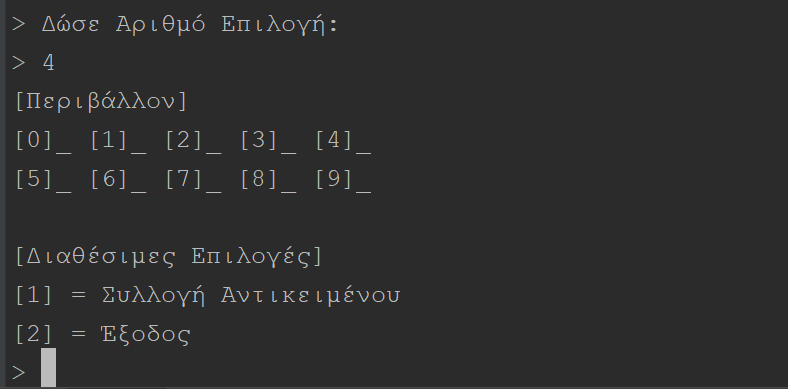
\includegraphics[width=1\textwidth]{image/2.2.PNG}
\end{center}

\noindent
Παρατηρεί ότι δεν υπάρχει τίποτα επόμενος επιλεγεί έξοδος και επιστρέφει στο αρχικό μενού.

\begin{center}
			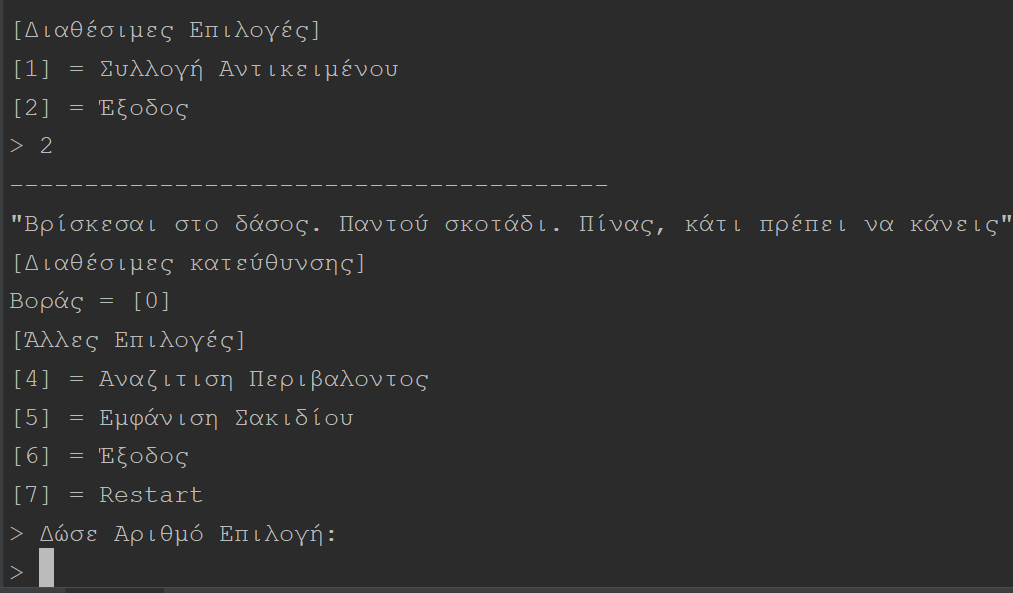
\includegraphics[width=1\textwidth]{image/2.3.PNG}
\end{center}


\noindent
Αποφασίζει να προχωρήσει και επιλεγεί των βορά από τις διαθέσιμες κατευθύνσεις
\begin{center}
			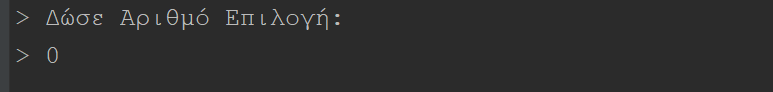
\includegraphics[width=1\textwidth]{image/2.4.PNG}
\end{center}

\noindent
στον νέο χώρο αποφασίζει να αναζητήσει το περιβάλλον πάλη.

\begin{center}
			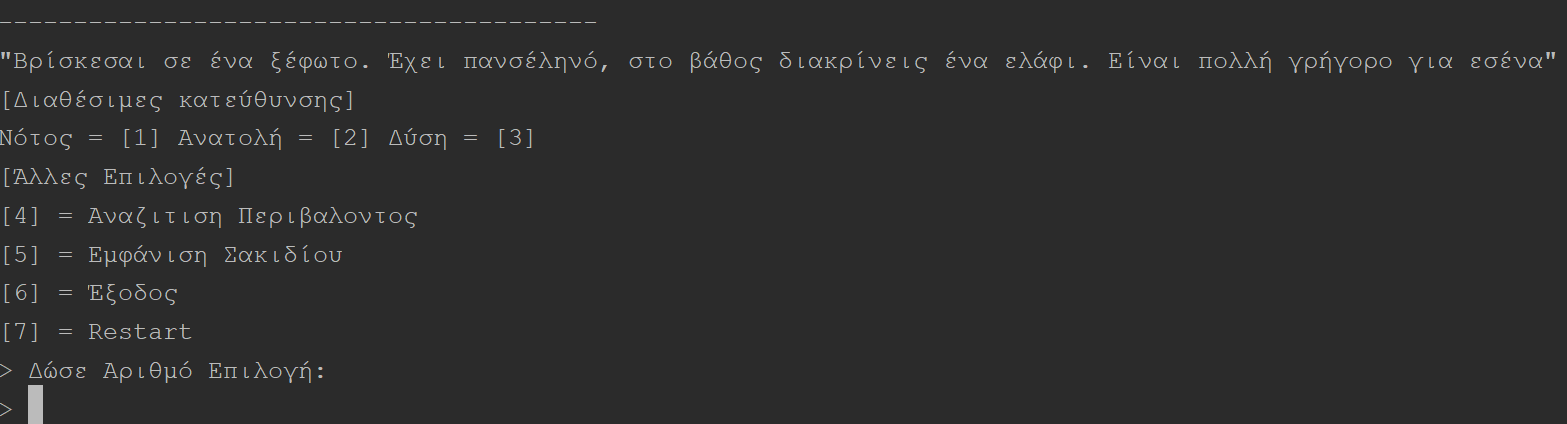
\includegraphics[width=1\textwidth]{image/2.5.PNG}
\end{center}

\begin{center}
			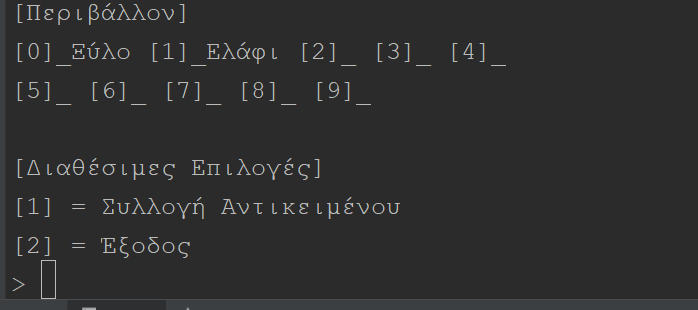
\includegraphics[width=1\textwidth]{image/2.6.PNG}
\end{center}
\noindent
Παρατηρεί ότι υπάρχουν διαθέσιμα αντικείμενα στο περιβάλλον. Αποφασίζει να 
συλλέξει το ξύλο. Επιλεγεί "Συλλογή Αντικείμενου", του ζητάει να επιλέξει ποιο αντικείμενο θέλει. Πληκτρολογεί 0 και το συλλέγει.

\begin{center}
			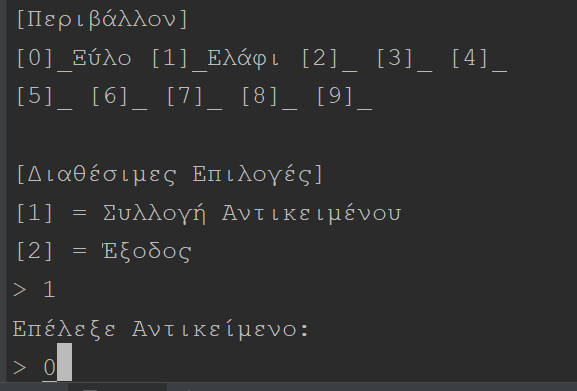
\includegraphics[width=1\textwidth]{image/3.1.PNG}
\end{center}

\noindent
Παρατηρούμε ότι το αντικείμενο χάθηκε από το περιβάλλων.
\begin{center}
			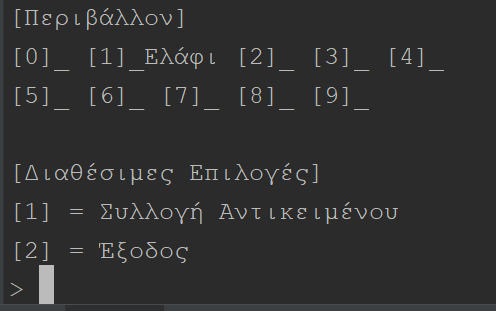
\includegraphics[width=1\textwidth]{image/3.2.PNG}
\end{center}

\noindent
Επιλεγεί έξοδο και επιστρέφει στο αρχικό μενού.
\begin{center}
			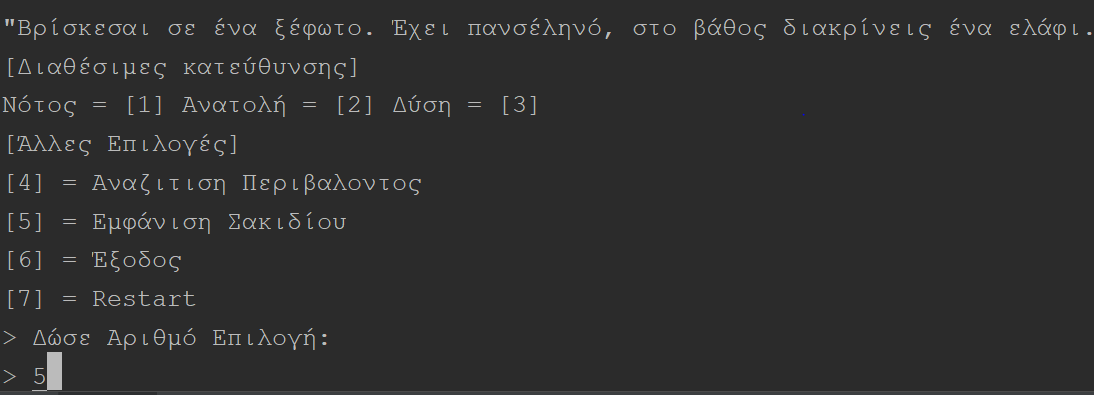
\includegraphics[width=1\textwidth]{image/3.3.PNG}
\end{center}

\noindent 
Επιλεγεί να δει το σακίδιο του.
\begin{center}
			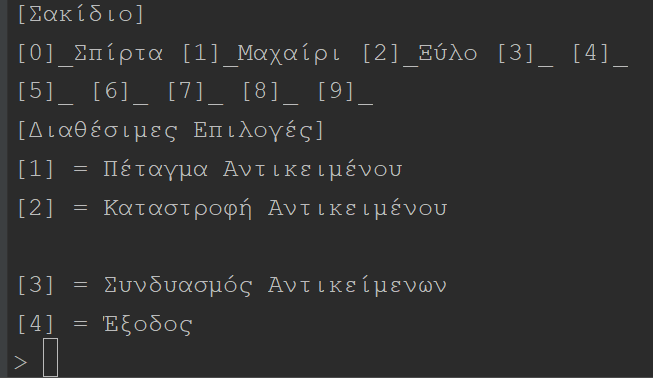
\includegraphics[width=1\textwidth]{image/3.4.PNG}
\end{center}
\noindent
Αποφασίζει να συνδυάσει δυο αντικείμενα από το σακίδιο
\begin{center}
			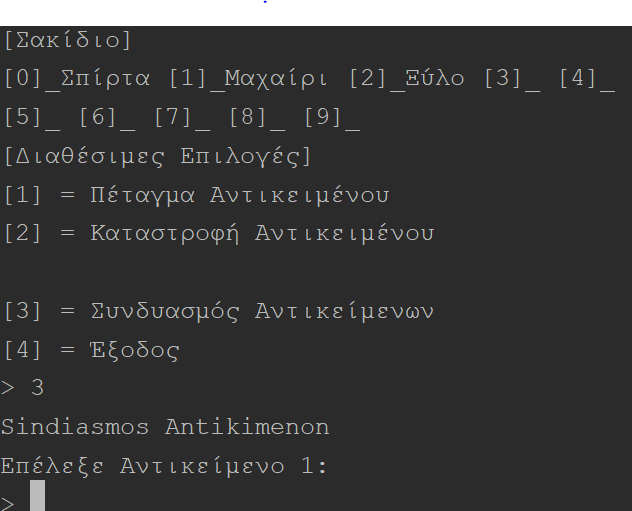
\includegraphics[width=1\textwidth]{image/3.5.PNG}
\end{center}

\noindent
Επιλεγεί το ξύλο και τα σπίρτα

\begin{center}
			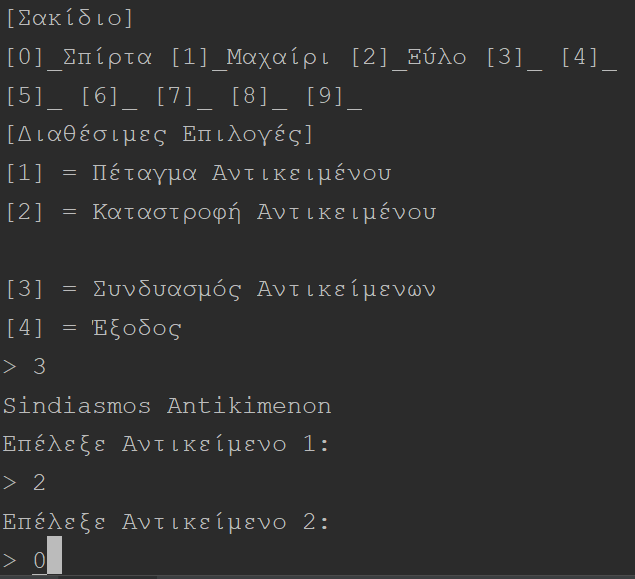
\includegraphics[width=1\textwidth]{image/3.6.PNG}
\end{center}

\noindent
Αυτά τα δυο αντικείμενα εξαφανιζόντανε και στην θέση τους εμφανίζετε το αντικείμενο φωτιά.

\begin{center}
			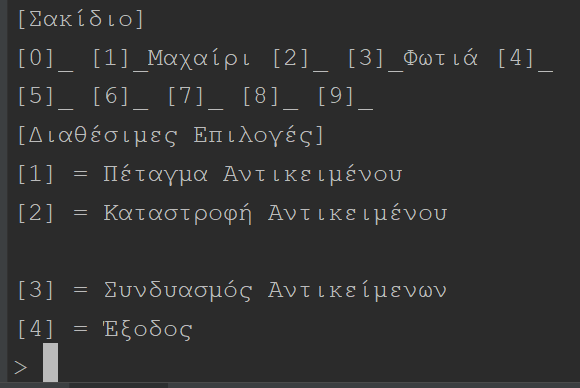
\includegraphics[width=1\textwidth]{image/3.7.PNG}
\end{center}


\textbf{*(Λόγω του μεγάλου φόρτου των εξετάσεων δεν προλαβαίνω να τελειώσω το documendation)}
\end{document}